\documentclass{article}
\usepackage[utf8]{inputenc}
\usepackage[ngerman]{babel}

% Convenience improvements
\usepackage{csquotes}
\usepackage{enumitem}
\setlist[enumerate,1]{label={\alph*)}}
\usepackage{amsmath}
\usepackage{amssymb}
\usepackage{mathtools}
\usepackage{tabularx}

\usepackage{csquotes}

% Proper tables and centering for overfull ones
\usepackage{booktabs}
\usepackage{adjustbox}

% Change page/text dimensions, the package defaults work fine
\usepackage{geometry}

\usepackage{parskip}

% Drawings
\usepackage{tikz}
\usepackage{forest}

% Adjust header and footer
\usepackage{fancyhdr}
\pagestyle{fancy}
\fancyhead[L]{Multimedia --- \textbf{Blatt 2}}
\fancyhead[R]{Laurenz Weixlbaumer (11804751)}
\fancyfoot[C]{}
\fancyfoot[R]{\thepage}
% Stop fancyhdr complaints
\setlength{\headheight}{12.5pt}

\newcommand{\Deltaop}{\, \Delta\, }
\newcommand{\xor}{\, \oplus\, }

\begin{document}

\paragraph{Convolution Filter}

Ein Convolution Filter wird für die (künstliche bzw. nachträgliche) Reduktion oder Erhöhung der Schärfe von Bildern verwendet. Das Eingabebild wird als Matrix von Farb- und Helligkeitswerten interpretiert. Ein sog. Kernel, eine kleine benutzerdefinierte Matrix, wird schrittweise \enquote{über} das Bild geschoben. Jeder Pixel nimmt einen Wert in Abhängigkeit von benachbarten Pixeln, skaliert durch die Werte des Kernels, an.

\begin{minipage}[t]{.45\textwidth}
    Bei einem Kernel von
    \vspace{.5em}
    \begin{center}
        \begin{tabular}{c c c}
            1 & 1 & 1 \\
            1 & 1 & 1 \\
            1 & 1 & 1 \\
        \end{tabular}
    \end{center}
\end{minipage}\hfill
\begin{minipage}[t]{.45\textwidth}
    \ldots und einem Bild das in Matrixform als
    \vspace{.5em}
    \begin{center}
        \begin{tabular}{c c c c c c}
            0 & 0 & 0 & 0 & 0 & 0 \\
            0 & 1 & 1 & 1 & 1 & 0 \\
            0 & 1 & 0 & 0 & 1 & 0 \\
            0 & 1 & 0 & 0 & 1 & 0 \\
            0 & 1 & 1 & 1 & 1 & 0 \\
            0 & 0 & 0 & 0 & 0 & 0 \\
        \end{tabular}
    \end{center}
    \vspace{.5em}
    dargestellt wird,
\end{minipage}

w\"urde der Kernel nun \"uber die Bildmatrix geschoben, wobei jeweils \"ubereinanderliegende Elemente miteinander multipliziert werden. Der Bildpixel in der Mitte des Kernels nimmt nun den Durchschnitt dieser Produkte an.

\begin{minipage}[t]{.3\textwidth}
    \begin{center}
        \begin{tabular}{c c c c c c}
            \emph{0} & \emph{0} & \emph{0} & 0 & 0 & 0 \\
            \emph{0} & \boxed{\emph{1}} & \emph{1} & 1 & 1 & 0 \\
            \emph{0} & \emph{1} & \emph{0} & 0 & 1 & 0 \\
            0 & 1 & 0 & 0 & 1 & 0 \\
            0 & 1 & 1 & 1 & 1 & 0 \\
            0 & 0 & 0 & 0 & 0 & 0 \\
        \end{tabular}
    \end{center}
\end{minipage}
\begin{minipage}[t]{.3\textwidth}
    \begin{center}
        \begin{tabular}{c c c c c c}
            0 & \emph{0} & \emph{0} & \emph{0} & 0 & 0 \\
            0 & \emph{1} & \boxed{\emph{1}} & \emph{1} & 1 & 0 \\
            0 & \emph{1} & \emph{0} & \emph{0} & 1 & 0 \\
            0 & 1 & 0 & 0 & 1 & 0 \\
            0 & 1 & 1 & 1 & 1 & 0 \\
            0 & 0 & 0 & 0 & 0 & 0 \\
        \end{tabular}
    \end{center}
\end{minipage}
\begin{minipage}[t]{.3\textwidth}
    \begin{center}
        \begin{tabular}{c c c c c c}
            0 & 0 & \emph{0} & \emph{0} & \emph{0} & 0 \\
            0 & 1 & \emph{1} & \boxed{\emph{1}} & \emph{1} & 0 \\
            0 & 1 & \emph{0} & \emph{0} & \emph{1} & 0 \\
            0 & 1 & 0 & 0 & 1 & 0 \\
            0 & 1 & 1 & 1 & 1 & 0 \\
            0 & 0 & 0 & 0 & 0 & 0 \\
        \end{tabular}
    \end{center}
\end{minipage}
\begin{minipage}[c]{.05\textwidth}
    $\cdots$
\end{minipage}

Die jeweiligen Ergebniswerte im Beispiel sind $\frac{1}{3}$, $\frac{4}{9}$ und $\frac{4}{9}$. Dieser Prozess wird f\"ur alle Elemente der Bildmatrix wiederholt.

\emph{Beispiel angelehnt an https://iq.opengenus.org/convolution-filters/.}

\paragraph{High- und Low-Resolution}

Die Aufl\"osung eines Bilds im Rasterformat ist definiert durch die Anzahl der Pixel die das Bild darstellen. Ein Bild mit einer Aufl\"osung von 5000x5000 ist hochaufl\"osender als ein Bild mit einer Aufl\"osung von 1000x1000.

Bei der Einbindung von Bildern in Webseiten ist es oft sinnvoll die Aufl\"osung so niedrig wie m\"oglich zu w\"ahlen. So sind niedrigaufl\"osende Bilder gut geeignet als Thumbnails. Hier f\"allt die niedrige Aufl\"osung bei den \"ublicherweise kleinen Darstellungsgr\"ossen nicht sonderlich auf, aber die Dateigr\"osse kann drastisch kleiner sein. Bei Bildern die in voller Bildschirmgr\"osse angezeigt werden, kann es sinnvoll sein das Bild in der Bildschirmaufl\"osung (also \"ublicherweise recht hochaufl\"osend) anzuzeigen um die bestm\"ogliche Qualit\"at zu erreichen.

Das wird auch in Zukunft sinnvoll bleiben, keine unn\"otig grossen Daten zu laden ist immer gut.

\paragraph{Aliasing-Effekte}

Aliasing-Effekte treten in Bildern auf wenn die Sampling-Rate zu hoch ist, wenn also die Aufl\"osung unter einem gewissen kritischen Punkt ist. Dann erscheinen etwa eigentlich unterschiedlich aussehende Elemente als gleich, wie im folgenden Beispiel erkenntlich ist.

\begin{minipage}[t]{.49\textwidth}
    \centering
    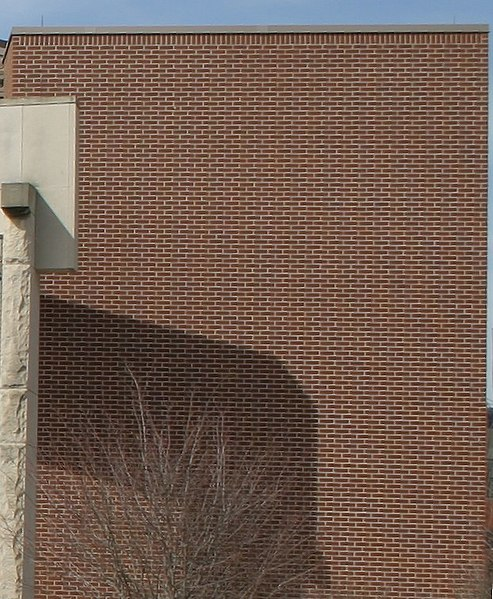
\includegraphics[width=.7\textwidth]{aliasing_ex_1.jpg}
\end{minipage}
\begin{minipage}[t]{.49\textwidth}
    \centering
    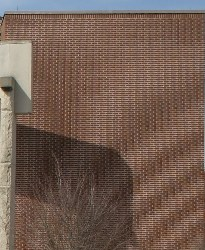
\includegraphics[width=.7\textwidth]{aliasing_ex_2.jpg}
\end{minipage}

\emph{Beispielbilder entlehnt aus https://en.wikipedia.org/wiki/Aliasing.}

\paragraph{JPEG}

\begin{enumerate}
    \item Es folgt eine grobe Erl\"auterung der Kompressionsschritte des JPEG-Formats.
    
    \begin{enumerate}[label=\arabic*)]
        \item Farbtransformation in YCbCr (Y = Luminanz, CbCr = Chrominanz --- blau und rot) Farbraum
        \item Downsampling der Chrominanzinformationen.
        \item Diskrete Kosinustransformation in 8x8 Bl\"ocke.
        \item Normalisierung der durch DCT erhaltenen Bl\"ocke anhand einer Normalisierungstabelle die bei Kompression anzugeben ist und im komprimierten Bild enkodiert ist. (Elementweise Division.)
        \item Kodierung der nun erhaltenen Daten, etwa durch Huffman-Kodierung.
    \end{enumerate}

    \item Nach der diskreten Kosinustransformation und Normalisierung haben Zellen mit niedrigem Spalten- bzw. Zeilenindex \"ublicherweise h\"ohere Werte als solche mit hohen Indices. Bei hohen Spalten- und Zeilenindices sammeln sich Nullen. Durch das \enquote{zigzag} Auslesen sammeln sich die Nullen am Ende, damit verbessert sich die Komprimierbarkeit der Daten im vergleich zum vertikalen oder horizontalen Auslesen.
    
    \item Verlustbehaftete Kodierung wegen der Normalisierung.
\end{enumerate}

\end{document}
